\cotefile{35}
\scanpage{2}
\noindent\hfill\margin{\handwritten{back to G.}}\par

\noindent SGA 7\qquad Monodromy Group in Algebraic Geometry

\reversemarginpar
\noindent\margin{\handwritten{Grothendieck}}I\quad G\deleted{\unsure{ad|ed}}eneralities on the local monodromy g\deleted{o}roup. The monodromy theorem by arithmetic means.

\noindent\margin{\handwritten{Grothendieck}}II\quad Case of solvable\deleted{s} action\deleted{s} of a fundamental group (variant of the \deleted{group} monodromy theorem).

\noindent\margin{\handwritten{Grothendieck}}III\quad The monodromy theorem by geometric means.\normalmarginpar
\margin{\handwritten{\figure{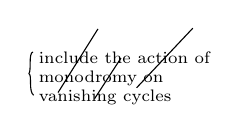
\begin{tikzpicture}[x=1cm,y=1cm,scale=.86,transform shape]
\node[anchor=north west,align=left,inner sep=0pt,font=\scriptsize] at (.14,.06)
{\deleted{include the action of}\\
 \deleted{monodromy on}\\
 \deleted{vanishing cycles}};
\draw (.06,.05) .. controls (-.01,.03) and (.04,-.22) .. (0,-.27)
 .. controls (.05,-.29) and (-.01,-.53) .. (.07,-.59);
\draw (.43,-.55)--(1.02,.39) (.97,-.64)--(1.36,-.04) (1.59,-.48)--(2.42,.40);
\end{tikzpicture}}}}

\reversemarginpar
\noindent\margin{\handwritten{Grothendieck}}IV\quad General properties of the groups of vanishing cycles. Case of isolated singul\deleted{\unsure{ei|ee}}ar points of the special fiber.

% slanted
\noindent\margin{\handwritten{Grothendieck\par
\figure{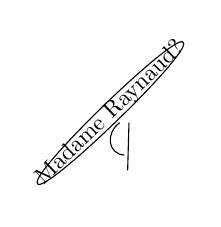
\begin{tikzpicture}[scale=.84,transform shape]
\begin{scope}[rotate=44,transform shape]
\node[inner sep=1.1pt] (q) {Madame Raynaud?};
\draw (q.west) .. controls (q.north west) and ([xshift=3pt]q.north east) .. (q.east)
 .. controls (q.south east) and ([xshift=-3pt]q.south west) .. (q.west);
\end{scope}
\draw (q.south) .. controls +(-.21,-.15) and +(-.26,.02) .. ++(.07,-.49);
\draw ([xshift=4pt]q.south) -- ++(-.02,-.72);
\end{tikzpicture}}}}V\quad Monodromy group acting on the fundamental group: theorems of tame action and of essentially tame action.

\noindent\margin{\handwritten{Madame Raynaud\par\deleted{Madame Raynaud}}}\deleted{VI}\handwritten{\inserted{\unsure{App.|Arr.}}}\quad Application: finite presentation of the geometric\unsure{s} fundamental groups

\noindent\margin{\handwritten{\uline{Rim}}}\handwritten{\inserted{$\underline{\overline{\mathrm{VI}}}$\quad Formal moduli (is with Deligne)}}

\noindent\margin{\handwritten{Grothendieck}}VII\quad Biextensions of sheaves of groups.

\noindent\margin{\handwritten{Grothendieck}}\handwritten{\inserted{$\underline{\overline{\mathrm{VIII}}}$\quad Extensions and biextensions of group schemes \unsure{by|by} $G_m$}}

% The outlined typescript above this line has a downward point between the two words.
\noindent\margin{\handwritten{Grothendieck}}\deleted{\unsure{VIII}}\handwritten{$\underline{\overline{\mathrm{IX}}}$}\quad Application\handwritten{s} to the Néron model: \deleted{the} theorem \tikz[baseline,remember picture]{\coordinate (orthogpoint);}
\tikz[overlay,remember picture]{
\node[anchor=south west,inner sep=2pt] (orthogtext) at ([xshift=-1.55cm,yshift=.38cm]orthogpoint) {\inserted{of orthogonality, theorem}};
\draw (orthogtext.north west) .. controls ([xshift=-.28cm]orthogtext.north west) and ([xshift=-.28cm]orthogtext.south west) .. (orthogtext.south west)
 -- ([xshift=-.13cm,yshift=.33cm]orthogpoint) -- ([yshift=-.13cm]orthogpoint)
 .. controls ([yshift=.22cm]orthogpoint) and ([xshift=.10cm,yshift=.32cm]orthogpoint) .. ([xshift=.25cm,yshift=.33cm]orthogpoint)
 -- (orthogtext.south east) .. controls ([xshift=.25cm]orthogtext.south east) and ([xshift=.25cm]orthogtext.north east) .. (orthogtext.north east);
} of semi-stable reduction.\handwritten{\tikz[baseline]{\draw[line cap=round] (.01,.045)--(.045,.020) (.11,.035)--(.155,.025) (.23,.059)--(.28,.046);}}

\noindent\margin{\handwritten{\deleted{Deligne}}}
\figure{\resizebox{\linewidth}{!}{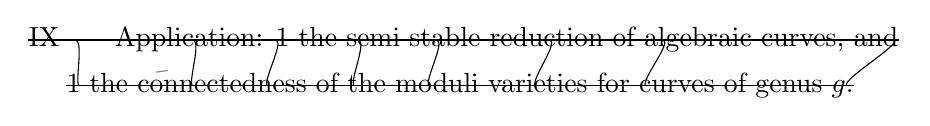
\begin{tikzpicture}
\node[anchor=west,inner sep=0pt] (a) at (0,0) {\deleted{IX}\qquad \deleted{Application: {\deleted{\illegible{1} the}} semi-stable reduction of algebraic curves, {\deleted{and}}}};
\node[anchor=west,inner sep=0pt] (b) at (.48,-.58) {\deleted{{\deleted{\illegible{1} the}} \tikz[overlay]{\draw[gray] (.24,.26)--(.39,.28);}connectedness of the moduli varieties for curves of genus $g$.}};
\draw (a.west) -- (a.east);
\draw (b.west) -- (b.east);
\foreach \p/\q in {.055/.016,.19/.16,.285/.255,.38/.365,.47/.46,.60/.595,.73/.735,.995/.99}
{\path (a.west) -- (a.east) coordinate[pos=\p] (t);
 \path (b.west) -- (b.east) coordinate[pos=\q] (u);
 \draw (t) .. controls +(0.09,-.05) and +(-.04,.09) .. (u);}
\end{tikzpicture}}}

% archive sheet number: 1
